\documentclass[10pt,a4paper]{article}

\sloppy
\usepackage{caption}
\usepackage{subcaption}
\captionsetup{font = footnotesize, labelfont = bf}
\captionsetup[sub]{font=scriptsize,labelfont= bf}
\setlength{\textwidth}{16cm}
\setlength{\textheight}{23cm}
\addtolength{\hoffset}{-1.5cm}
\addtolength{\voffset}{-1.5cm}
\setlength{\headheight}{35pt}
\usepackage[utf8]{inputenc}
%\usepackage[spanish]{babel}
\usepackage[spanish,es-tabla]{babel}
\usepackage{ae}
\usepackage{graphicx}
\usepackage{wrapfig}
\usepackage{tikz,pgfplots}
\usepackage{epsfig}
%\usepackage{multicol, array}
\usepackage{amsmath}
\usepackage{amssymb, amsthm}
\usepackage{amsfonts}
\DeclareMathOperator\erf{erf}
\theoremstyle{definition}
%\newtheorem*{definition}{Definición}
%\newtheorem*{example}{Ejemplo}
%\newtheorem*{theorem}{Teorema}
%\usepackage{epsdice}
\usepackage{tcolorbox}
\tcbuselibrary{theorems}

\newtcbtheorem[auto counter,number within=section]{theorem}{Teorema}%
{colback=green!5,colframe=green!35!black,fonttitle=\bfseries}{th}

\newtcbtheorem[auto counter,number within=section]{definition}{Definición}%
{colback=blue!5,colframe=blue!35!black,fonttitle=\bfseries}{def}

\newtcbtheorem[auto counter,number within=section]{example}{Ejemplo}%
{colback=red!5,colframe=red!35!black,fonttitle=\bfseries}{ej}


%\numberwithin{equation}{chapter}
\usepackage{euscript}
\usepackage{mathrsfs}
\usepackage{sectsty}
\usepackage{lipsum}
\usepackage{courier}
\usepackage{listings}
\usepackage{xcolor}
\definecolor{verde}{rgb}{0.0, 0.5, 0.1}
\lstset{%
  language=R, literate =  {á}{{\'a}}1 {é}{{\'e}}1 {í}{{\'{\i}}}1 {ó}{{\'o}}1 {ú}{{\'u}}1 {Á}{{\'A}}1 {É}{{\'E}}1 {Í}{{\'I}}1 {Ó}{{\'O}}1 {Ú}{{\'U}}1 {ü}{{\"u}}1 {Ü}{{\"U}}1 {ñ}{{\~n}}1 {Ñ}{{\~N}}1,
  backgroundcolor=\color{gray!6!},
  classoffset=0,
  basicstyle=\ttfamily\scriptsize\bfseries,
  showspaces=false,
  showstringspaces=false,
  keywordstyle=\color{blue!60!black}\bfseries,
  stringstyle=\color{blue},
  numbers=none,
  numberstyle=\ttfamily\small,
  commentstyle=\color{verde}\textbf,
  morecomment=[l][\color{verde}\textbf],
  frame = single,
  framexleftmargin= -0pt,
  framexrightmargin= -5pt}




\usepackage{fancyhdr}

\decimalpoint
\usepackage[T1]{fontenc}
%\usepackage{textcomp}

\pagestyle{fancy}
\lhead{Lic. en Física - Física Experimental I \\ U.N.S.L. - Depto. de Física}
\rhead{
\includegraphics[width=1cm]{graf/unsl.jpg}}
%\pagenumbering{arabic}
%\setcounter{page}{1}
\setlength{\parskip}{3mm}

\pgfplotsset{compat=1.13}

\usepackage{hyperref}
\hypersetup{
    colorlinks=true,
    linkcolor=blue,
    filecolor=black,      
    urlcolor=blue,
    citecolor=black,
   	anchorcolor=black
}
 
\urlstyle{same}



\begin{document}

\begin{center}
{
\begin{large}
\textbf{Laboratorio N$^o$ 2} \\
\vspace*{0.1cm}
 \textbf{Calibrando un inclinómetro digital}

\textbf{(usando el acelerómetro de 3 ejes del celular)}
\end{large}
}
\end{center}

\subsection*{¿Qué significa calibrar un instrumento?}


\begin{itemize}
\item[$\bullet$] Calibrar es comparar una señal con un patrón, para que la señal nos permita estimar una medida. En este caso, la señal será la salida del acelerómetro de un teléfono celular, mientras que el patrón estará constituído por ángulos calculados mediante medidas de longitud.
\item[$\bullet$] Habitualmente la señal es de distinta magnitud que el patrón.
\item[$\bullet$] Cuando se utiliza un rango de la señal, lo que buscamos es una curva de calibración, es decir, una función que nos entregue la medida buscada una vez obtenida la señal.
\end{itemize}


\subsection*{Acelerómetro del teléfono.}

Casi cualquier teléfono celular tiene lo que llamamos un acelerómetro de tres ejes, es decir, que mide aceleraciones en las tres dimensiones. Un acelerómetro consta de un resorte impreso en metal de tamaño muy pequeño (ver Fig.(\ref{acelerometro})) que, mediante medidas eléctricas, es capaz de sensar las fuerzas que actúan sobre la masa. Cuando el resorte se estira o se comprime, la longitud varía, y esta variación se traduce en aceleración mediante medidas capacitivas. 

\begin{figure}[h]
\centering
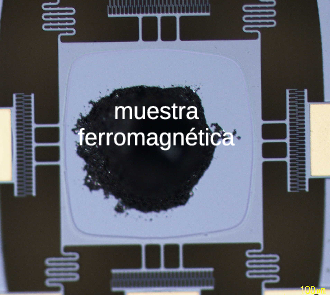
\includegraphics[height=0.4\textwidth]{graf/acelerometro}
\caption{Sensor del tipo de los acelerómetros de los teléfonos, diseñado en el Laboratorio de Bajas Temperaturas y sistemas micro-electro-mecánicos, UNSL.  \label{acelerometro}}
\end{figure}


Los teléfonos celulares cuentan con tres acelerómetros ortogonales (ver Fig.(\ref{telefono})). Cuando el teléfono está en reposo, el acelerómetro descompone la gravedad en sus tres ejes. Esta descomposición es la que permite que el software del teléfono rote la pantalla cuando el teléfono se mueve. Es justamente esta descomposición la que utilizaremos para estimar el ángulo respecto de la horizontal del teléfono, lo que nos permitirá medir ángulos en un futuro.


\begin{figure}[h]
\centering
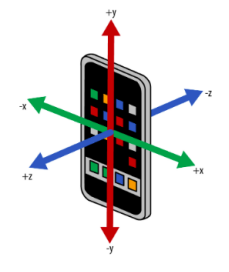
\includegraphics[height=0.4\textwidth]{graf/telefono}
\caption{Direcciones ortogonales en las cuales miden los acelerómetros de los teléfonos.  \label{telefono}}
\end{figure}


\subsection*{Aplicación para obtener los datos}

Hay un sinfin de aplicaciones para Android que \textit{loggean} los datos del acelerómetro, sin embargo, elegimos \href{https://play.google.com/store/apps/details?id=pt.acoelhosantos.android.acc}{Accelerometer Data Recorder} porque es la más simple disponible, y garantiza una salida limpia --sin ningún filtro-- y la máxima frecuencia de muestreo disponible (obviamente, dependiendo de la configuración de la aplicación).

Los datos del acelerómetro son exportados a archivos \texttt{'.tsv'}, con un formato de columnas:

\noindent \texttt{'nro-fila \textbackslash t marca-temporal(ms) \textbackslash t ax \textbackslash t ay \textbackslash t az \textbackslash t nombre-archivo \textbackslash n'}

\noindent donde \texttt{'\textbackslash t'} es la separación de las columnas (un \texttt{tab}) y \texttt{'\textbackslash n'} es el fin de línea de \texttt{UNIX} (todos los Linux y casi todos los lenguajes de programación).

Es importante notar que todas las personas en el curso deben usar la misma aplicación, ya que el formato de los \textit{data-sets} no es un tema menor a la hora de compartir información. En caso de querer cambiar por otra aplicación, deberán ponerse de acuerdo.

\section{Actividad: Modelo, montaje y experimento de prueba}

\subsection{Modelo}

Ya dijimos que el acelerómetro en reposo descompone a $g$ en tres componentes. Entonces, el teléfono en posición \textit{horizontal} ($\theta = 0$), poseerá una descomposición de $g$, $g_h = g_{h,x} \mathbf{e_1} + g_{h, y}\mathbf{e_2} + g_{h,z} \mathbf{e_3}$, donde $\{\mathbf{e_i}\}$ con $i = 1,2,3$ son los vectores ortonormales de la base del acelerómetro.

Es posible pensar que, al inclinar el teléfono, tendremos \textit{otra} descomposición de la aceleración de la gravedad $g_\theta = g_{\theta ,x} \mathbf{e_1} + g_{\theta, y}\mathbf{e_2} + g_{\theta,z} \mathbf{e_3}$.

El producto punto o escalar entre los vectores $g_h$ y $g_\theta$ deberá proveernos de una forma de obtener el ángulo $\theta$, que no es otra cosa que el ángulo entre diferentes descomposiciones de la gravedad, es decir, el ángulo de inclinación del telégono respecto de la horizontal.

\textbf{Responder por escrito} 

\noindent \textbf{a)} Realice un esquema del teléfono en reposo con el vector $\vec{g}$, primero en posición horizontal ($\vec{g}_h$) y luego inclinado un ángulo $\theta$ ($\vec{g}_{\theta}$).

\noindent \textbf{b)}  Utilizando el producto punto, calcule el ángulo $\theta$ como función de las componentes de $g_h$ y $g_\theta$, mencionadas anteriormente.

\noindent \textbf{c)} Inspeccionando la fórmula anterior, deduzca el intervalo de $\theta$ que será posible obtener a partir de las componentes de $\vec{g}_{h}$ y $\vec{g}_\theta$.


\subsection{Medidas de longitud y ángulos: cómo montar esto}

\begin{figure}[h]
\centering
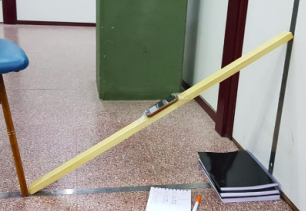
\includegraphics[height=0.4\textwidth]{graf/plano}
\caption{Teléfono sobre plano inclinado, del cual quiere conocerse el ángulo de inclinación. Es importante no perturbar con vibraciones el teléfono, mientras dura la medida. Los acelerómetros responden fuertemente a las vibraciones, siendo uno de los sensores preferidos para detectarlas.}
\label{plano}
\end{figure}

En la Fig.\eqref{plano}, se muestra la configuración experimental a utilizar:

\begin{itemize}
\item[$\bullet$] El teléfono está montado (con cintas adhesivas) sobre una tabla de madera plana, que sirve de soporte (puede utilizarse una tabla proveniente de un cajón de verdulería). Esta madera forma un triángulo rectángulo con la pared y el suelo.
\item[$\bullet$] Sobre la pared y el piso se encuentran adheridas con cinta dos reglas metálicas, que permiten medir las longitudes de los catetos opuesto y adyacente del triángulo rectángulo. En caso de no contar con reglas largas, pueden utilizarse cintas métricas ó utilizar reglas de 30 cm y disminuir el largo de la tabla de madera.
\item[$\bullet$] A fin de no demorar mucho --por experiencia se lo decimos-- es \textit{menester} que la tabla sea mantenida en su lugar en cada medida, mediante algún método de sujeción (una silla en este caso, aunque puede ser un libro pesado, un ladrillo, etc...)
\end{itemize}


\subsection{Experimento de prueba}
\begin{itemize}

\item[a)] Monte la configuración experimental mencionada.

\item[b)] Mida el ángulo del plano inclinado utilizando trigonometría y midiendo distancias (medidas reales, no redondee).

\item[c)] Tome uno o dos segundos de medidas para la posición horizontal ($g_h$) y, luego, para un ángulo conocido mediante las longitudes de los catetos (obteniendo $g_\theta$). Realice los cálculos del modelo utilizando las medias de cada componente de $g$, y como incerteza el $SEM$ (limpie datos y haga las cosas pertinentes a fines de no \textit{sesgar} la media). 

\item[d)] Compare las magnitudes obtenidas en los puntos (b) y (c). 
\end{itemize}

\section{Actividad: Mediciones}

\subsection{Medidas de longitud y del acelerómetro}
En esta actividad vamos a repetir las medidas que hicimos anteriormente, pero para un rango de valores (es decir, para una calibración confiable).

\begin{itemize}
\item[a)] Realice la primera muestra con $\theta =0$, es decir, horizontal (apoyado en el piso). Registre un número algo mayor a 2000 medidas sin perturbar el teléfono. Nombre este archivo (en la aplicación) como \texttt{00.tsv}. 

\item[b)] Haga lo mismo para cada uno de los ángulos:

$\theta_i = \frac{\pi}{18} \;\,  , \frac{2\pi}{18} \;\, , \frac{3\pi}{18} \;\, , \frac{4\pi}{18} \;\, , \frac{5\pi}{18} \;\, , \frac{6\pi}{18} \;\, , \frac{7\pi}{18} \;\, , \frac{8\pi}{18} = 10^o, 20^o,30^o,40^o,50^o,60^o,70^o,80^o$

\vspace{2mm}

\item[c)]utilice los nombres de archivo \texttt{01.tsv}, \texttt{02.tsv},...,\texttt{08.tsv} para enumerar las medidas.

\item[d)] En cada medida, registre las longitudes de los catetos, a fines de calcular el ángulo $\theta_{l}$ para cada una de las posiciones en las que se coloca el acelerómetro.
\end{itemize}




 Algunas consideraciones:
 
\begin{itemize}
\item[$\bullet$] Para acelerar el proceso: mida la longitud de la madera y calcule, en base a los valores de $\theta$ pedidos, las longitudes de uno de los catetos para cada $\theta$. Con esta lista de longitudes en la mano, es más fácil demorar media hora en lugar de dos.
\item[$\bullet$] Intente abarcar el mayor rango posible ($10^o$ a $80^o$) (pero no caiga en la locura): si los extremos resultan difíciles o las reglas no alcanzan, reduzca el rango sin perder puntos de medida.
\item[$\bullet$] Obviamente, cada uno de los valores de $\theta$ propuestos es \textit{aproximado}: podemos admitir variaciones de $3^o$ ó más.
\end{itemize}


\section{Actividad: Análisis de datos}

\begin{small}
\textbf{Nota:} \emph{Vamos a hacer todos los análisis de datos el miércoles en clase. Cada estudiante deberá tener los archivos} \texttt{tsv} \emph{del teléfono, nombrados como se indica en este texto} (\texttt{1.tsv,2.tsv,...,8.tsv}) \emph{y otro csv con los catetos, y el ángulo calculado por trigonometría}.
\end{small}

Teniendo en cuenta que vamos a utilizar muchos datos, es conveniente tener un arreglo de datos tipo \textit{Tidy-Data}, un forma usual --entre otras-- de arreglar datos, pensada para lenguajes vectorizados como \texttt{R} o \texttt{Python}. En el Apéndice se muestra el \textit{Tidy-Data}, junto con otro par de funciones de \texttt{R} para manejar arreglos grandes. Pedimos encarecidamente no caer en el manejo de 10 variables separadas, y llenar de líneas repetidas el código, sino intentar sistematizar las operaciones. 

\subsection{Medidas de longitud}

Calculando ángulos e incertezas con las medidas de longitud.

\begin{itemize}
\item[a)] Obtenga los ángulos $\theta_{l}$ a partir de las medidas de longitud.
\item[b)] Obtenga la incerteza $\delta \theta_{l}$ a partir de las medidas de longitud.
\item[c)] Informe los valores extremos de $\delta \theta_l$, y discuta sus posibles causas ¿Acaso las incertezas en las medidas de longitud no son iguales? ¿qué hace que cambien los valores de $\delta \theta_l$? 
\end{itemize}


\subsection{Medidas del acelerómetro}

Calculando dispersiones de ángulos y cuantificando una medida a partir de los datos del acelerómetro.

\begin{itemize}
\item[a)]  Tenga en cuenta que hay que cargar 9 archivos ASCII. Utilice el código provisto en el Apéndice para hacerlo. Asegúrese que el código recorte los datasets a $2000$ medidas por cada archivo, o recortarlos en las operaciones. 

\item[b)] Calcule los ángulos $\theta_{a}$ a partir de hacer las operaciones necesarias sobre las medidas de $g_h$ y cada uno de los $g_\theta$. La idea de propagar la incerteza puede ser difícil, y buscaremos cuantificar la incerteza a partir de la dispersión de $2000$ valores de $\theta_a$ calculados de cada ángulo. Pueden perderse algunos valores en el cálculo de los ángulos, pues utilizamos una función trigonométrica inversa.

\item[c)] Calcule para cada ángulo la media muestral, la desviación estándar de la muestra y el $SEM$. Informe los ángulos con la mayor y la menor $s_\theta$ (desviación estándar de la muestra). Haga histogramas de las dos medidas anteriores. Discuta posibles orígenes de la discrepancia entre los valores de $s_\theta$.

\item[d)] ¿Qué probabilidades tiene \textit{una medida} del acelerómetro, de caer en el intervalo $\overline{\theta} \pm s_\theta$? (Informe esto para los valores extremos de $s_\theta$)

\item[e)] ¿Qué probabilidades tiene \textit{la media $\overline{\theta_{a}}$ (2000 repeticiones)} del acelerómetro, de caer en el intervalo $\overline{\theta_a} \pm SEM$? (Informe esto para los valores extremos de $s_{\theta}$ del punto anterior)

\end{itemize}




\subsection{Comparando medidas}

Ahora vamos a comparar las medidas, pero en lugar de hacerlo para una medida, lo vamos a hacer para todos los puntos encontrados.

\begin{itemize}
\item[$\bullet$] Con las medidas de longitud, debemos tener un \texttt{data.frame} que tenga tres columnas: $\theta_l \, , \delta \theta_l \, , N$, donde $N$ es el número de medida.
\item[$\bullet$] En el acelerómetro utilizaremos la media muestral de los datos limpios, $\overline{\theta_{a}}$ como estimador de tendencia central, y el $SEM$ como desviación estándar de $\overline{\theta_{a}}$. Debemos obtener un \texttt{data.frame} con las columnas: $\theta_{a} \, , SEM\, , N$. Este arreglo de datos debe tener solamente $N$ datos, pues consta de medias y no de todos los datos. 
\end{itemize}

Si unimos estos datos, podremos graficar $\theta_{a}$ (en el eje $y$) \textit{vs.} $\theta_l$. La gráfica de los puntos debe parecer una recta $\theta_{a} = \theta_l$, es decir, una recta de pendiente $1$.

\begin{itemize}
\item[$\bullet$] Grafique $\theta_{a}$ \textit{vs.} $\theta_l$.
\item[$\bullet$] Grafique, encima del gráfico anterior, una recta de pendiente unitaria.
\item[$\bullet$] Haga la diferencia $\delta \theta = \theta_l - \overline{\theta_{a}}$ y grafique $\delta \theta$ \textit{vs.} $\theta_l$, adjuntando a $\overline{\theta_a}$ barras indicando el $SEM$. Informe el rango de $\delta \theta$. Discuta dónde la medida del acelerómetro funciona mejor y dónde funciona peor. Evalúe si $\delta \theta$ es menor a tres $SEM$ para todas las medidas. 
\end{itemize}



\pagebreak

\section*{Apéndice: \textit{Tidy-Data} y medidas del acelerómetro}


Se tienen catorce [infinitas] colecciones de datos provenientes del acelerómetro de un celular, almacenadas en los archivos \texttt{00.tsv,01.tsv,...,13.tsv}. Estas medidas se utilizaron para \textit{calibrar} el celular como un \textit{inclinómetro}, es decir, a partir de las medidas del acelerómetro se obtienen ángulos de inclinación del celular, como puede observarse en la Fig.\eqref{plano}.


Cada archivo posee medidas del teléfono en reposo, buscando medir el ángulo de inclinación del teléfono sobre un plano inclinado el cual se varió de inclinación para cada medida. 

Cada uno de los archivos tiene:

\begin{itemize}
\item[$\bullet$] Una cantidad de filas no necesariamente igual al resto de los archivos.
\item[$\bullet$] Seis columnas (sin nombre en cada archivo), a saber:
\begin{enumerate}
\item \texttt{Número de Fila}
\item \texttt{Tiempo de la Medida}
\item \texttt{$g_x$}
\item \texttt{$g_y$}
\item \texttt{$g_z$}
\item \texttt{Nombre de archivo sin extensión (nosotres usaremos números enteros, indicando el número de medida)} 
\end{enumerate}
\end{itemize}

Si bien se pueden escribir tantas líneas de código como archivos se tengan, a veces resulta engorroso, y otras veces titánico. Claramente, es preferible utilizar un solo \texttt{data.frame} por cuestiones operativas. Para esto es necesario colocar todos los archivos en un directorio particular, definiéndolo luego como el directorio de trabajo.

\begin{lstlisting}[language = R]
#Preliminares: librerías y directorios de trabajo
cat("\014")
rm(list = setdiff(ls(), lsf.str()));
rm(list=lsf.str());

#Carpeta de laburo
setwd("/home/juan/Documentos/Docencia/fexpi/2019/Laboratorios/Laboratorio4/Datos/")

#nombres de los archivos en un vector "char" 00.tsv,01.tsv,02.tsv,...,13.tsv
nombres <- list.files(pattern = ".tsv") #elige sólo los archivos con extensión '.tsv'(tab separated values)
\end{lstlisting}

Hasta acá se tiene cada nombre de archivo en el vector \texttt{nombres}. Ahora es necesario leer cada archivo, cargarlo en una variable, y luego apilarlos en un \texttt{data.frame}. Para esto usamos un bucle \texttt{for} y la función \texttt{rbind(x,y)} que apila las filas de \texttt{data.frames} \texttt{x} e \texttt{y} si tienen los mismos nombres de columnas.

\begin{lstlisting}[language = R]
acel <- data.frame(NULL)
for(i in 1:length(nombres)){
acel <- rbind(acel, read.csv(file = nombres[i], header = F, sep = "\t",
            colClasses = c("integer", "numeric", "numeric", "numeric","numeric", "integer" )))
}
\end{lstlisting}

\noindent el parámetro \texttt{colClasses()} en la función \texttt{read.csv} indica la clase de cada columna. No es necesario especificarlo, pero puede acelerar mucho la carga de datos en conjuntos de datos grandes.

Ahora podríamos descartar la primera columna de \texttt{acel}, porque es información que no tiene sentido (son los números de fila en cada archivo \texttt{.tsv}). Lo mismo con el tiempo de la medida (segunda columna), ya que no estamos buscando ninguna dinámica en los datos. También definimos el nombre de las columnas luego de quitarle las dos primeras:

\begin{lstlisting}[language = R]
acel <- acel[ ,c(-1,-2)] #saca columnas 1 y 2
colnames(acel) <- c("ax", "ay", "az", "Med")
\end{lstlisting}

\noindent con lo anterior, obtenemos finalmente un \texttt{data.frame} arreglado como \textit{tidy data}, es decir, cada variable está en una columna. A las variables de aceleración las apodamos \textit{cuantitativas}), mientras que aquellas variables como el número de medida las apodamos \textit{variables categóricas}, en este caso, un marcador que separa las medidas (sí, es un número, pero simplemente marca el orden en el que se hicieron las medidas y no tiene otro sentido que separar medidas).

Este tipo de datos, \textit{tidy data}\footnote{Puede consultarse Wickham, H. (2014). Tidy Data. Journal of Statistical Software, 59(10), 1 - 23. doi:http://dx.doi.org/10.18637/jss.v059.i10}, es \textit{una} de algunas formas de arreglar datos. Las ventajas que presenta este tipo de arreglo de datos es que nos permitirá limpiar, operar y hacer estimaciones con \textit{cada una de las medidas} (en este caso), utilizando bucles o funciones similares.

Por otra parte, si no se ordenan los datos \textit{de alguna manera}, las chances de error de cálculo --por equivocaciones-- se multiplican, por no hablar de el tiempo de cálculo. Las estructuras de datos, como se ve, también tienen su semántica, y es bueno aprender a manejarse con una lógica definida en lugar de hacer todo caótico (aunque siempre hacer cosas de alguna forma es mejor que no hacer nada).




\subsection{Ángulo por medio de los catetos}

En el archivo \texttt{angulosmed.csv} podemos suponer que se tienen:

\begin{itemize}
\item \texttt{Longitud Cateto opuesto}
\item \texttt{Longitud Cateto adyacente}
\item \texttt{$\delta$ de la medida de longitud}
\item \texttt{$\theta_l$}
\item \texttt{$\delta \theta_l$}
\item \texttt{Número de Medida (con $\theta_l = 0$ para $N = 0$)}
\end{itemize}

\noindent donde los ángulos de inclinación $\theta_{l}$ (en radianes) del plano en el que se colocó el teléfono en cada medida (\texttt{Med}); estos ángulos fueron estimados mediante medidas de longitud de los catetos. El archivo se carga en el \texttt{data.frame} que llamamos \texttt{a} en lo que sigue, y tiene columnas de nombres \texttt{CO}, \texttt{CA}, \texttt{dL}, \texttt{angulo.l}, \texttt{d.angulo.l} y \texttt{Medida}. Notamos que \texttt{Medida} es el indice que vincula a los dos \texttt{data.frames} que tenemos (otro requisito del \textit{tidy data}: si se tienen distintos arreglos de datos, debemos tener una columna en común para operar con ellos).

En el \texttt{data.frame} con las aceleraciones, podemos mostrar una columna \texttt{ang.patron} que nos informe para cada medida de aceleración el ángulo estimado por medio de los catetos. Puede ser:

\begin{lstlisting}[language = R]
#agregar datos ángulo
ang.patron <- vector(mode = "numeric", length = nrow(acel)) #vector de largo del dataframe
for(i in 1:nrow(acel)){
ang.patron[i] <- a$angulo[a$Medida == acel$Med[i]]
}
acel$ang.patron <- ang.patron
rm(ang.patron)
\end{lstlisting}

\subsection{Seleccionando \textit{partes} del \texttt{data.frame} utilizando el número de medida}
Una de las ventajas de los datos ordenados, es que podemos \textit{seleccionar} partes del \texttt{data.frame}. Esto puede hacerse mediante el número de medida en el \texttt{data.frame} o mediante el ángulo que definimos anteriormente. Por ejemplo, si queremos calcular la \textit{media muestral} de $a_x$ para cada medida, entonces podemos escribir:

\begin{lstlisting}[language = R]
#calcular media de ax
mmuestral.ax <- vector(mode = "numeric", length = length(unique(acel$Med)))
for(i in 1:max(acel$Med)){
parte.acel <- acel[acel$Med == i, ] #selecciona las filas con Med = i  
mmuestral.ax[i] <- mean(parte.acel$ax)  #calcula la media de la selección
}
rm(parte.acel)
\end{lstlisting}



\end{document}
